\chapter{Evaluation}
In this chapter, we evaluate \textsf{Flycatcher} quantitatively by running \textsf{Flycatcher} with a series of benchmark programs and observing the results. In this experimental evaluation we are interested in examining some of \textsf{Flycatcher}'s features as well as assessing its overall success in terms of code coverage. We start by introducing the choice of benchmark programs, before presenting the experiments and finally discussing them.

% by using it to generate unit tests for a chosen set of programs and examining the results.
% First, we present a summary of the parameters available to \textsf{Flycatcher} users. We then explain our rationale and constraints in choosing the benchmark programs. Next, we describe the experiments and present the results for each program before discussing the results obtained.

\section{Choosing the benchmark suite}
In choosing a suite of programs for evaluating \textsf{Flycatcher} we had the following objectives in mind:

\begin{itemize}
   \item Demonstrating \textsf{Flycatcher}'s ability to infer primitive types
   \item Demonstrating \textsf{Flycatcher}'s ability to infer user-defined types
   \item Demonstrating that \textsf{Flycatcher} works with methods of various size, complexity and arity
   \item Demonstrating \textsf{Flycatcher}'s ability to achieve high coverage for various methods in a reasonable time
\end{itemize}

However the constraints imposed to us by the current limitations of the \textsf{Flycatcher} application, made finding benchmark tests difficult. The constraints are the following:

\begin{itemize}
   \item \textsf{Flycatcher} does not handle the inference of \texttt{Array} parameters
   \item \textsf{Flycatcher} does not handle the inference of \texttt{Function} parameters
\end{itemize}

The reason why these constraints made it difficult to find benchmark programs is that array parameters are commonplace and because functions are first-class objects in JavaScript, they frequently occur as parameters too. This also indirectly imposed a restriction on the size of the benchmark programs --- most significant libraries and modules make use of either arrays or functions as parameters at some point. This is also why established JavaScript benchmark suites such as SunSpider or the V8 benchmark suite couldn't be used.

% Nevertheless, we were still able to evaluate whether we accomplished what we initially set out to do: build an automatic test generator for a comprehensive \emph{subset} of the JavaScript language.
With these objectives and constraints in mind, the list of methods in table \ref{benchmarktests} was put together. Some of the programs are custom, many were found using \textsf{Node.js}'s open-source module registry \textsf{npm} and others were taken from the V8 performance benchmark suite.

\begin{table}[h]
\centering
\begin{tabular}{|l|l|c|c|}
\hline
\textbf{Class} & \textbf{Method} & \textbf{LOC} \\
\hline
\texttt{Triangle} & & \\
           & \textit{getType} & 38      \\
\hline
\texttt{LinkedList} & & \\
           & \textit{append} & 15       \\
           & \textit{remove} & 16       \\
           & \textit{prepend} & 12      \\
           & \textit{insertAfter} & 8   \\
           & \textit{insertBefore} & 8  \\
           & \textit{at} & 6            \\
\hline
\texttt{BinarySearchTree} & &     \\
           & \emph{add} & 49      \\
           & \emph{contains} & 26 \\
           & \emph{remove} & 147  \\
           & \emph{size} & 9      \\
\hline
\texttt{RedBlackTree} & &         \\
           & \emph{insert} & 22   \\
           & \emph{contains} & 14 \\
\hline
\texttt{SplayTree} & &             \\
           & \emph{splay} & 60 \\
           & \emph{insert} & 23 \\
           & \emph{remove} & 23 \\
           & \emph{findMax} & 10 \\
           & \emph{findGreatestLessThan} & 17 \\
\hline
\texttt{Luhn Algorithm} & &     \\
           & \emph{isValidIdentifer} & 40 \\
\hline
\texttt{Base 64} & &     \\
           & \emph{encode} & 45 \\
           & \emph{decode} & 50 \\
\hline
\texttt{SHA1} & &             \\
           & \emph{hash} & 72 \\
\hline
\texttt{Poker} & &                 \\
           & \emph{rankHand} & 437 \\
\hline
\end{tabular}
\caption{Benchmark methods}
\label{benchmarktests}
\end{table}

% \begin{table}[h]
% \centering
% \begin{tabular}{|l|l|c|}
% \hline
% \textbf{Class} & \textbf{Method} & \textbf{LOC} \\
% \hline
% \texttt{Triangle} & & \\
%            & \textit{getType} & 38      \\
% \hline
% \texttt{LinkedList} & & \\
%            & \textit{append} & 15       \\
%            & \textit{remove} & 16       \\
%            & \textit{prepend} & 12      \\
%            & \textit{insertAfter} & 8   \\
%            & \textit{insertBefore} & 8  \\
%            & \textit{at} & 6            \\
% \hline
% \texttt{BinarySearchTree} & &     \\
%            & \emph{add} & 49      \\
%            & \emph{contains} & 26 \\
%            & \emph{remove} & 147  \\
%            & \emph{size} & 9      \\
% \hline
% \texttt{RedBlackTree} & &         \\
%            & \emph{insert} & 22   \\
%            & \emph{contains} & 14 \\
% \hline
% \texttt{SplayTree} & &             \\
%            & \emph{splay} & 60 \\
%            & \emph{insert} & 23 \\
%            & \emph{remove} & 23 \\
%            & \emph{findMax} & 10 \\
%            & \emph{findGreatestLessThan} & 17 \\
% \hline
% \texttt{Luhn Algorithm} & &     \\
%            & \emph{isValidIdentifer} & 40 \\
% \hline
% \texttt{Base 64} & &     \\
%            & \emph{encode} & 45 \\
%            & \emph{decode} & 50 \\
% \hline
% \texttt{SHA1} & &             \\
%            & \emph{hash} & 72 \\
% \hline
% \texttt{Poker} & &                 \\
%            & \emph{rankHand} & 437 \\
% \hline
% \end{tabular}
% \caption{Benchmark methods}
% \label{benchmarktests}
% \end{table}

\subsection{Triangle types}
The \texttt{Triangle} example is used in many testing papers for automatic test generation. It takes three numerical inputs and determines whether they can form a triangle. If so, it returns the type of the triangle \emph{i.e.} whether it is equilateral, isoceles or scalene. This example was chosen because it demonstrates \textsf{Flycatcher}'s ability to narrow down the search space for good test programs, by using the same parameters more than once inside the generated tests. Without that ability, generating three numerical inputs out of the set of natural numbers so that they form an equilateral triangle would be extremely inefficient. No custom data generators with this class in the experiments.

\subsection{Doubly circular linked list}
The doubly circular linked list example was picked because it demonstrates \textsf{Flycatcher}'s ability to infer user-defined types as well as deal with parameters which are not used in the program under test itself. The circularity of this data structure also shows that \textsf{Flycatcher} handles scenarios where termination issues might arise in the context of test generation. The implementation used is from \textsf{computer-science-in-javascript}\footnote{"\url{https://github.com/nzakas/computer-science-in-javascript}"}.

\subsection{Binary trees}
A variety of binary trees were chosen as benchmarks because they present interesting control structures for code coverage, as well as the requirement that they infer a user-defined type: the type for the trees' nodes. The standard \texttt{BinarySearchTree} implementation is from \textsf{computer-science-in-javascript}\footnotemark[2]. The \texttt{RedBlackTree} (a self-adjusting BST) implementation is from \textsf{red-black-tree-js}\footnote{"\url{https://github.com/jeffreyolchovy/red-black-tree-js}"}. The \texttt{SplayTree} (a self-adjusting BST with quick retrieval of recently accessed nodes) implementation is part of the Google V8 benchmark suite\footnote{"\url{https://github.com/hakobera/node-v8-benchmark-suite}"}. No custom data generators were used with these programs.

\subsection{Luhn Algorithm}
The Luhn Algorithm is a checksum algorithm used to validate the format of credit card numbers. This example demonstrates the use of custom data generators in order to narrow down the search space for code coverage. We specify the following \texttt{RegExp} as the random string generator, which represents a string of digits which may contain a character as well (to also test with \texttt{NaN}): \texttt{[0-9]+a?}. The code can be found in \textsf{computer-science-in-javascript}\footnotemark[2].

\subsection{Base 64}
The \texttt{Base64} class simply encodes and decodes text strings to and from a radix-64 representation. This program was chosen to test the efficiency of code coverage of its control structures. Custom data generators were used to achieve full coverage, as non-ASCII parameters take a specific path in the \emph{encode} method, as do non-base-64 strings in the \emph{decode} method. The custom string generators are, therefore respectively, \texttt{\textbackslash w+\textbackslash u0100?} and \texttt{\textbackslash w+}.

\subsection{SHA1}
The \texttt{SHA1} algorithm generates a SHA-1 secure hash of a string. The implementation is taken from Chris Veness\footnote{"\url{http://www.movable-type.co.uk/scripts/sha1.html}"}.

\subsection{Poker}
The benchmark method with the most deeply nested structure is the \texttt{Poker} class's \emph{rankHand} method. It carries out hundreds of comparisons and calculations in order to return the absolute rank of a hand of cards in Texas Hold'em poker. The input thus has to conform to a hand of poker cards, which is defined in the program as a string of five characters. A custom string generator is thus used for that purpose, with the following regular expression: \texttt{[AKQJT98765432]\{5\}}. The code is from \textsf{node-poker}\footnote{"\url{https://github.com/mjhbell/node-poker}"}.

\section{Experiments}
All the experiments are carried out on Mac OS X v10.6 with a 2.4GHz Intel Core 2 Duo processor and 4GB of RAM. Any of the configurable parameters are either specified or their default value is used. The noteworthy default values are:

\begin{itemize}
   \item type inference delay: 20
   \item maximum sequence length: 10
   \item number generator: \texttt{\textbackslash d\{10,20\}}
   \item string generator: \texttt{\textbackslash t\{10,20\}}
\end{itemize}

\subsection{Effect of varying the type inference delay}
In this first experiment we analyse the effect of varying the type inference delay discussed in part \ref{typeinference} (see usage in section \ref{usage}). Let us recall that this delay is put in place in order for \textsf{Flycatcher} to make confident type inferences, based on enough data. If there is not enough data when type inference is attempted for a parameter, we consider that the type inference is \emph{unsuccessful}. In figures \ref{trianglebench} and \ref{bstbench}, we observe the relation between the type inference delay and unsuccessful type inferences for two methods from the benchmarking set, using an average over twenty runs.

\begin{figure}[h]
\hspace*{-0.5cm}
\centering
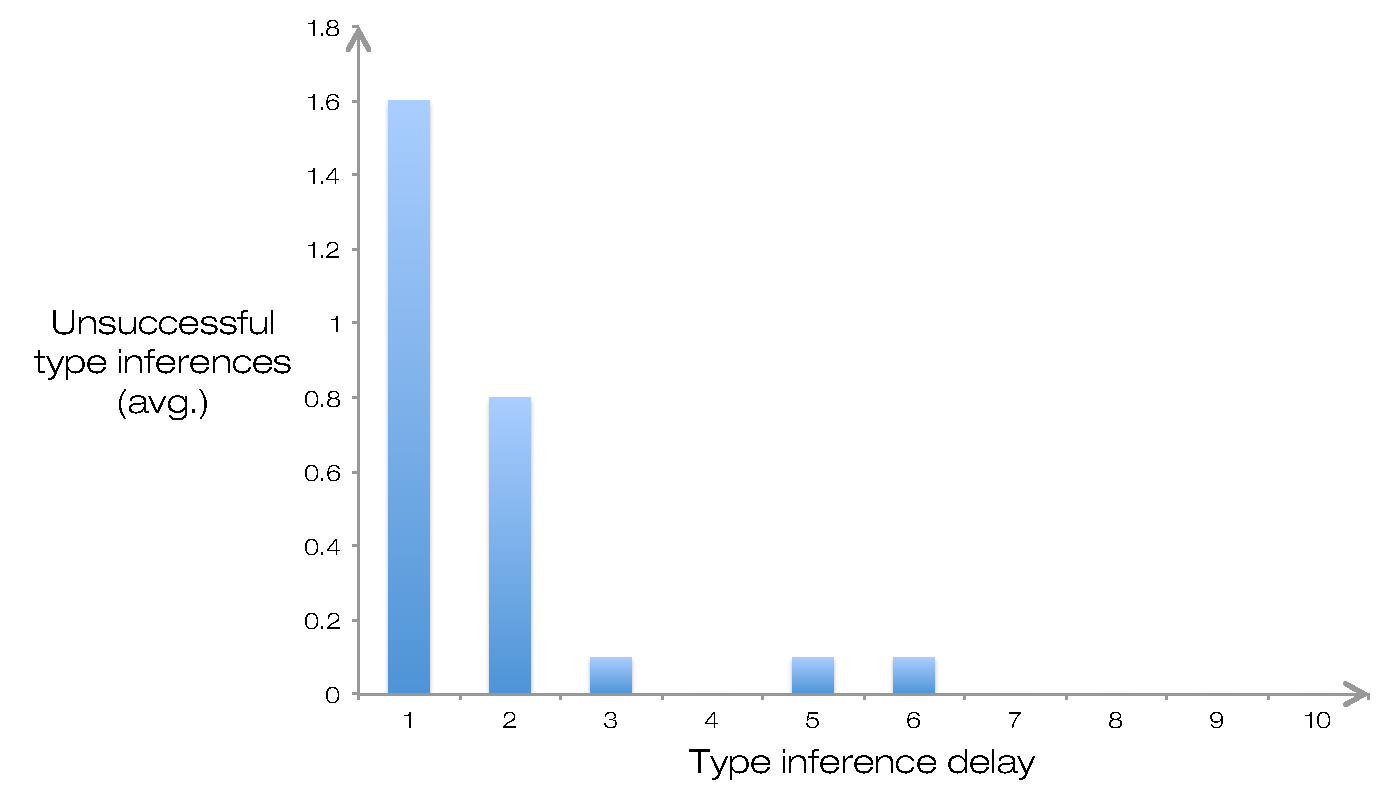
\includegraphics[scale=0.55]{./components/chapter7/triangle.pdf}
\caption{Results for method \texttt{Triangle.getType}}
\label{trianglebench}
\end{figure}

\begin{figure}[h]
\hspace*{-0.5cm}
\centering
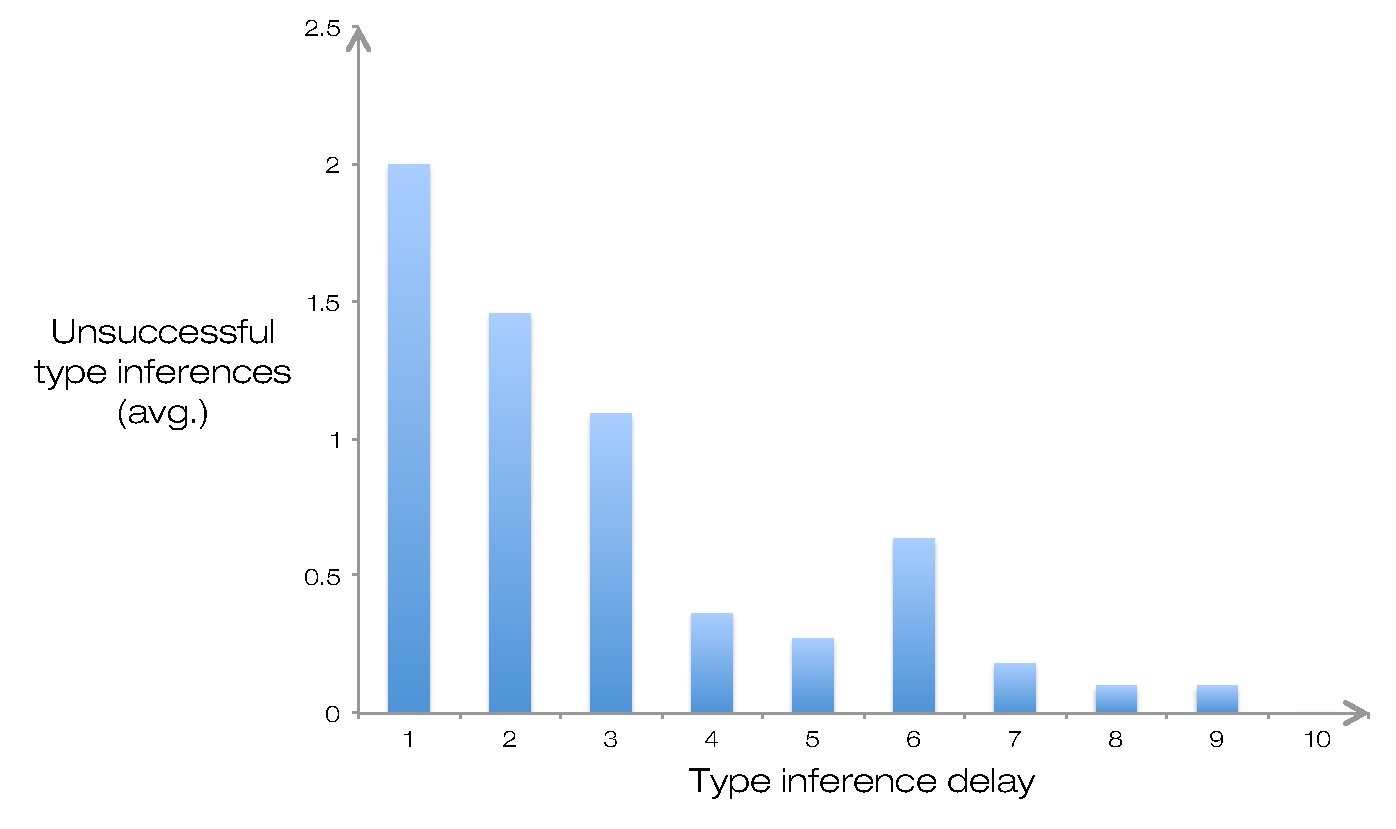
\includegraphics[scale=0.55]{./components/chapter7/bst.pdf}
\caption{Results for method \texttt{BinarySearchTree.add}}
\label{bstbench}
\end{figure}

\subsection{Effect of varying the length of tests}
In the second experiment, we vary the user-configurable variable that sets the length of method call sequences in tests (see usage in section \ref{usage}). We observe what the effect of modifying this variable is for all of the methods in the benchmark set. To give us a more comprehensive set of results to analyse, this process is carried out three times with varying `strict' timeouts of: 1 second, 5 seconds and 20 seconds. The results appear in figures \ref{1s}, \ref{5s} and \ref{20s} and each entry constitutes an average over 20 runs.

\begin{figure}[h]
\vspace*{-2.5cm}
\centering
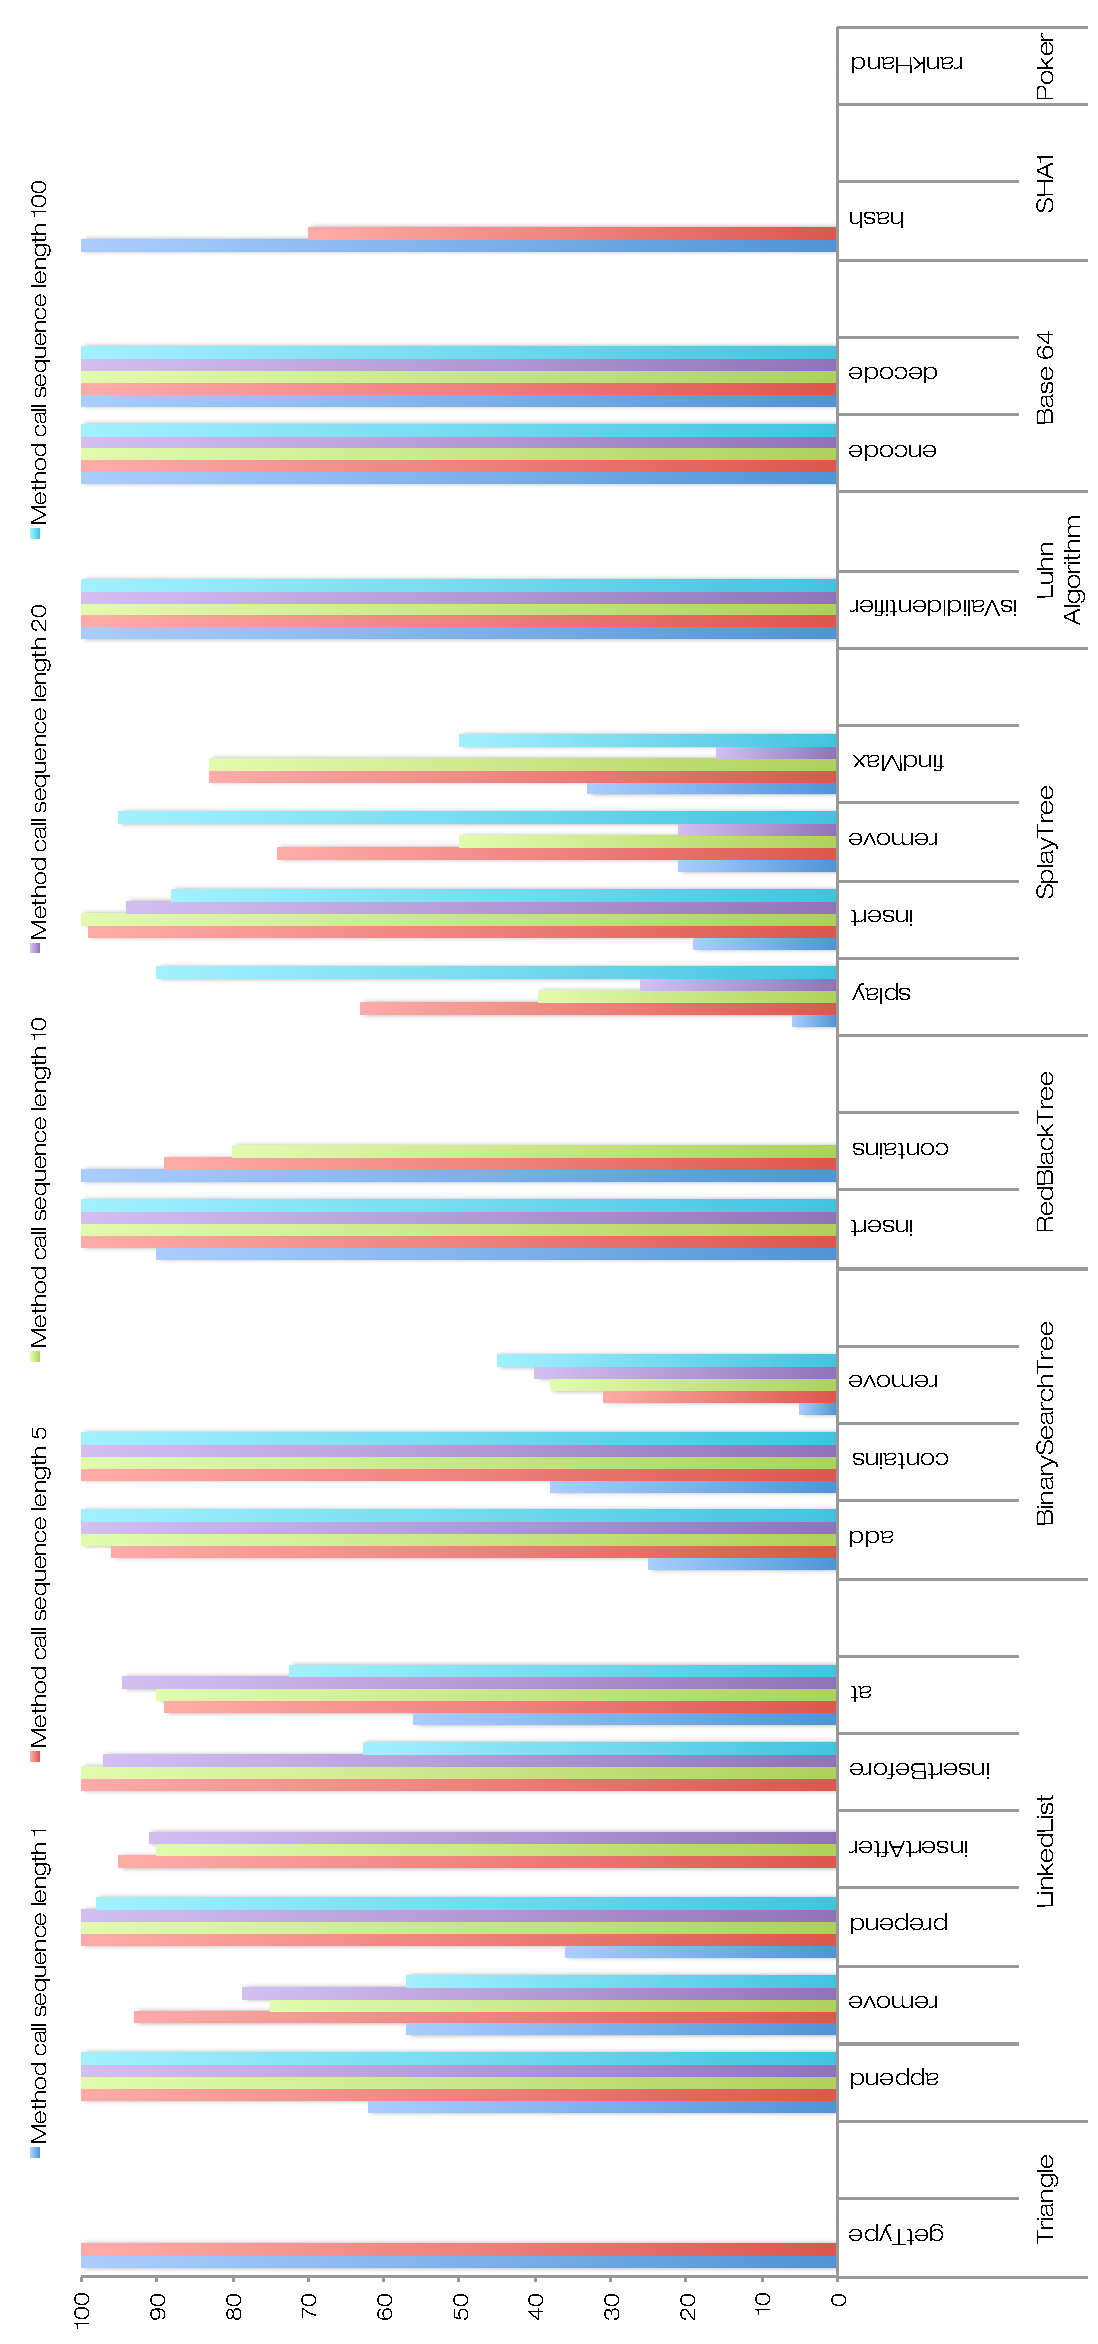
\includegraphics[scale=0.56]{./components/chapter7/1sr.pdf}
\caption{Results with 1s timeout}
\label{1s}
\end{figure}

\begin{figure}[h]
\vspace*{-2.5cm}
\centering
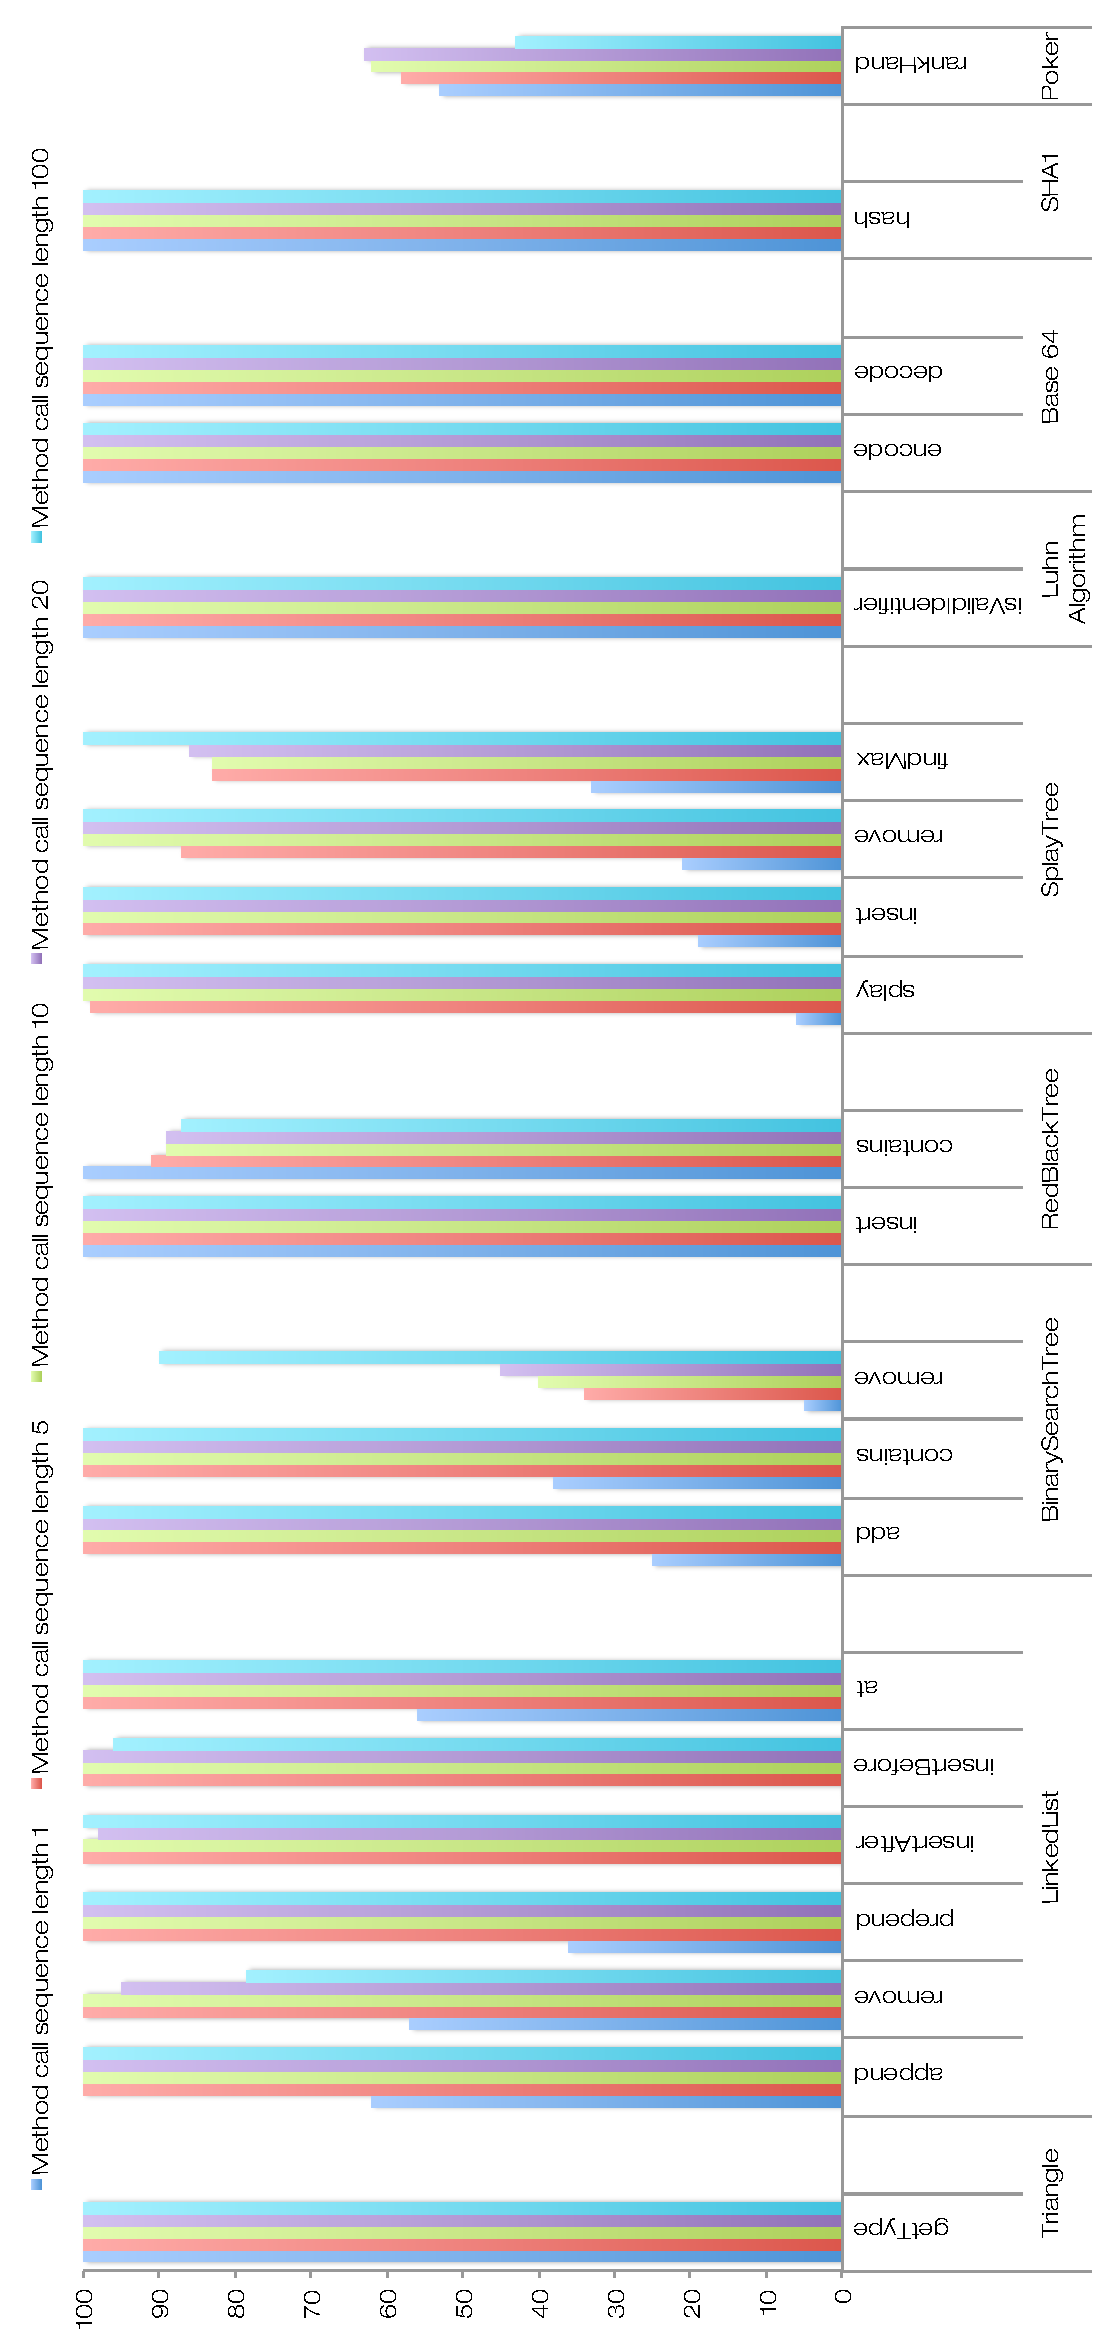
\includegraphics[scale=0.56]{./components/chapter7/5sr.pdf}
\caption{Results with 5s timeout}
\label{5s}
\end{figure}

\begin{figure}[h]
\vspace*{-2.5cm}
\centering
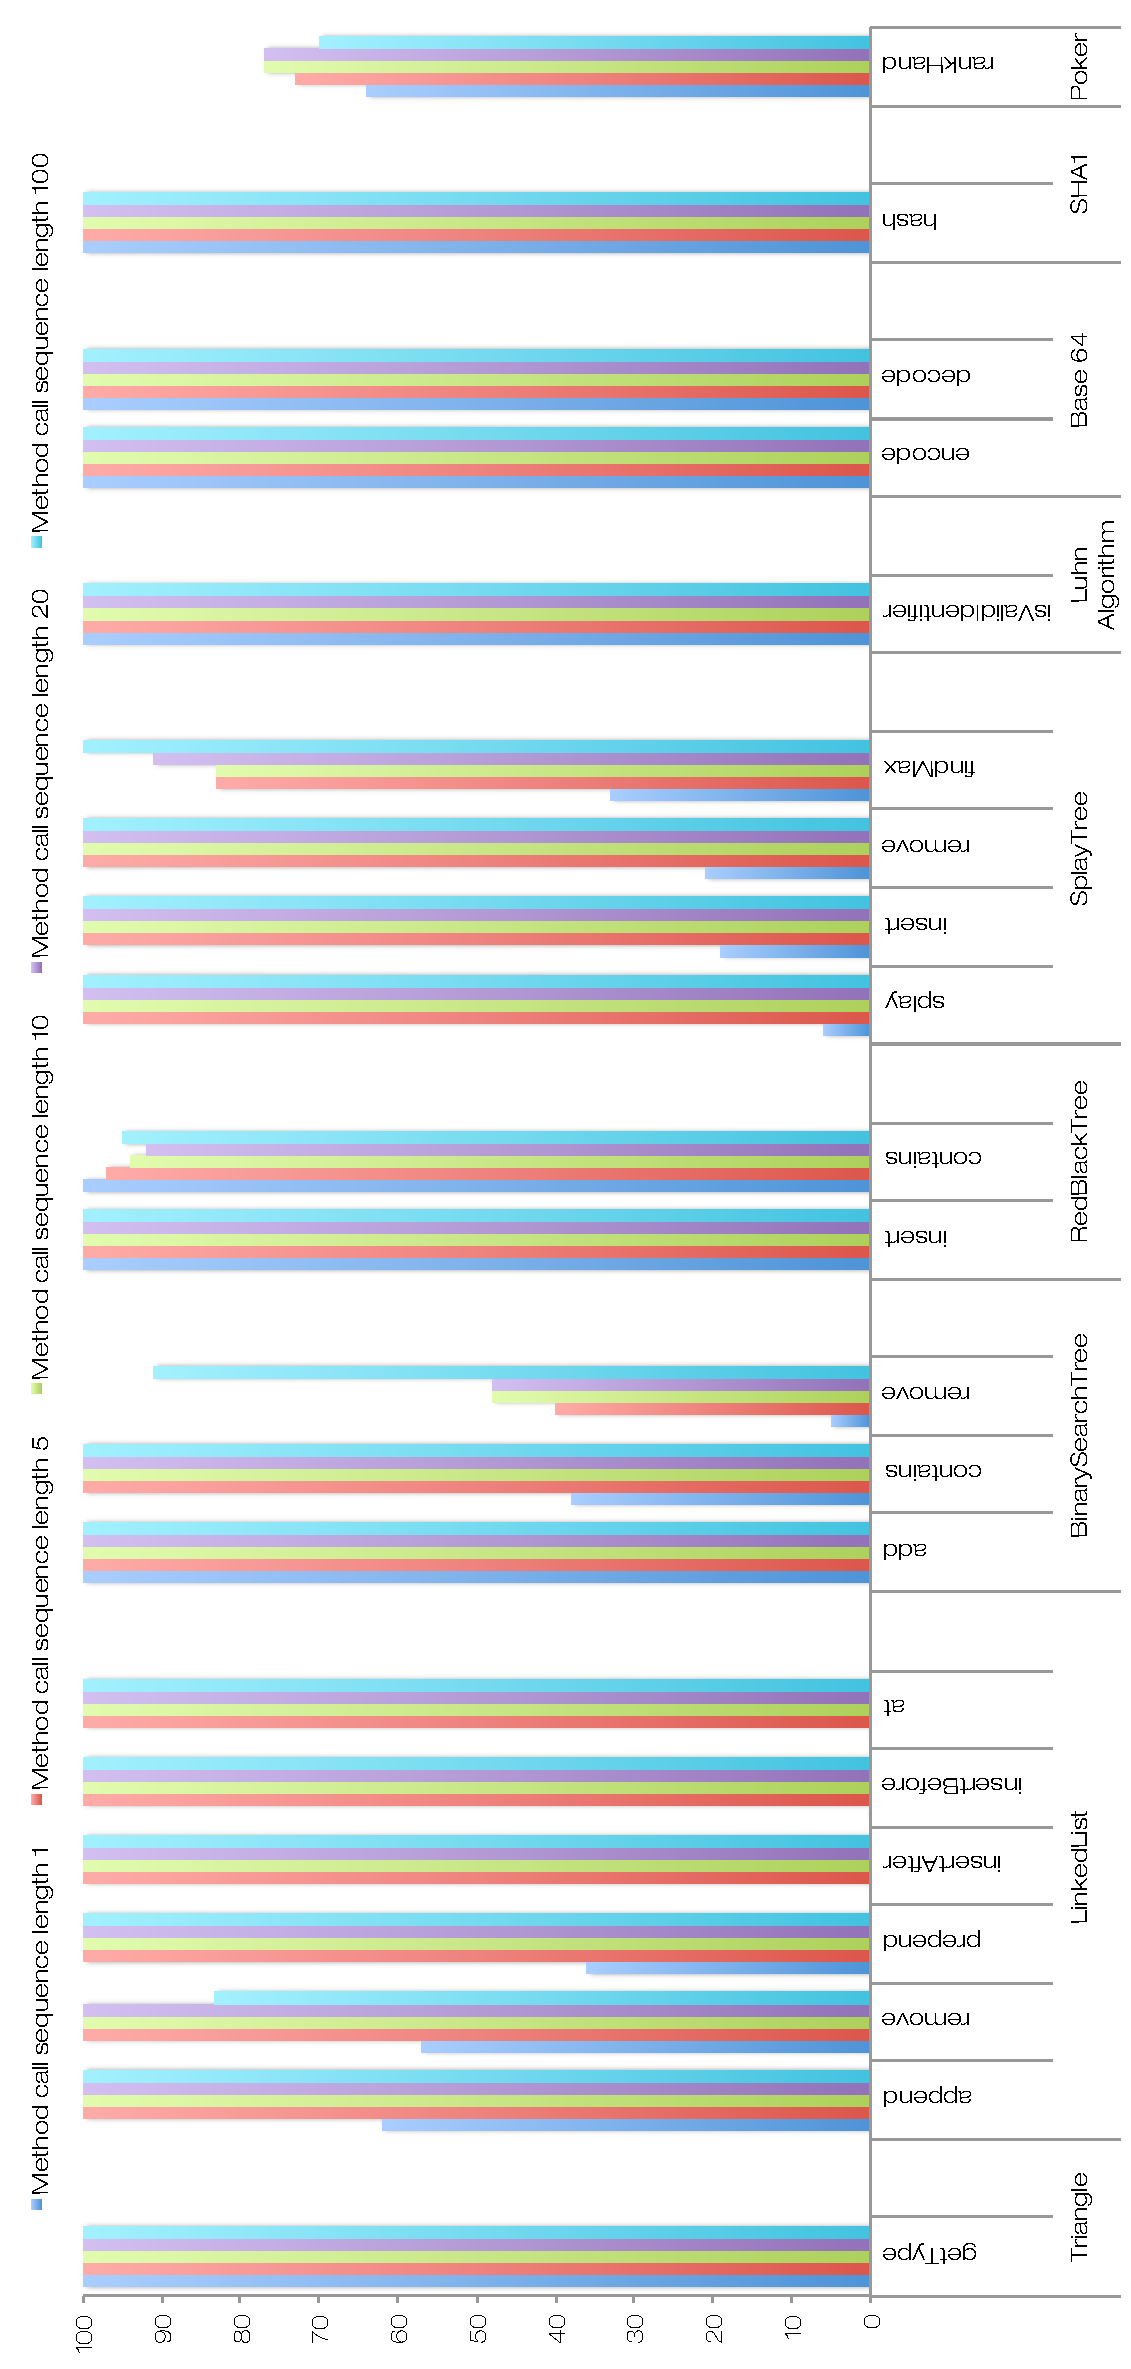
\includegraphics[scale=0.56]{./components/chapter7/20sr.pdf}
\caption{Results with 20s timeout}
\label{20s}
\end{figure}

\section{Discussion}
% talk about the problem of not having Fuction/Array and why they are difficult + the random has its limits
\begin{itemize}
   \item low inference delay leads to unsuccessful type inferences
   \item sometimes certain coverage simply \emph{cannot} be achieved with a certain length
   \item however the effect of length is highly variable, it speeds up but after at some point it slows down the test gen process --- hence why a search-based technique should be used as the random is not optimal (the optimal length is highly variable)
   \item random still achieves good results but it is helped by the custom data generators and the pooling system + our tests lend themselves well to that
   \item threats to validity: size of programs... + the fact that we don't deal with array or function as they are key js objects. discuss why we don't deal with them
   \item nonetheless based on what we set out to do, the work can be considered successful as full coverage is achieved for almost all methods in under 20 seconds, with a variety of different types and scenarios
\end{itemize}
